\chapter{Introduction}
\label{Chapter1}

%------------------------------------------------------------------------------

\section{Introduction}

Surveillance cameras have become popular and placed almost everywhere, e.g. train stations, airports, banks, shops, streets. The balance between security and privacy is an active subject for political/social debates. It is hard to keep a balance between security and privacy. A person may feel protected when he knows himself and his surroundings are being observed, but at the same time he may feel uncomfortable.

The information that people probably wants to know most about surveillance cameras is probably their viewing fields, e.g. where the cameras are, whether he is inside the area being observed. On the other hand, for indoor environment, because the space is usually small, people may easily locate the position and estimate the viewing fields of the cameras. For outdoor environment, it is rather hard to find surveillance camera systems hence they need special support to visually know the viewing fields in real scene. Fortunately, there is a technology which can be applied for this demand: Mixed Reality (MR). MR is encompassing both Augmented Reality and Augmented Virtuality, merging the real world in which we are living and the virtual world created by computers. MR can produce new environments where real and virtual entities can co-exist and interact in realtime \cite{Reference3}.

MR applications are traditionally equipped with Head Mounted Displays (HMD) as shown in figure \ref{fig:HMD}. However, HMDs are usually bulky and inconvenient for outdoor applications, where high-level mobility is crucial. In recent years, mobile devices have become popular, devices like cell phones, Personal Digital Assistants (PDA) can be seen everywhere. Their prices have come down and they could reach the hands of ordinary people even in developing countries like Viet Nam. High-end mobile devices, such as Apple iPhone and Google T-Mobile G1, usually have high specifications. As for their important advantages for outdoor MR applications, they are almost always equipped with built-in cameras, Global Positioning System (GPS), and accelerometer devices. These auxiliary devices usually meet the requirements on building up outdoor MR applications because they can provide video and information to help estimating position and orientation of the mobile devices \cite{Reference2} \cite{Reference4}.

\begin{figure}[htbp]
	\centering
	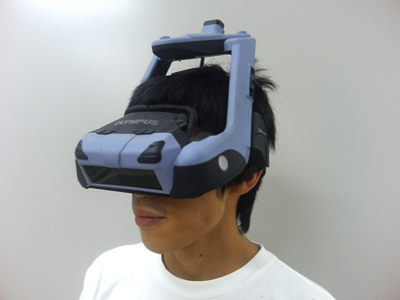
\includegraphics{./Primitives/hmd.jpg}
	\rule{35em}{0.5pt}
	\caption[Head Mounted Dislay]{A Head Mounted Dislay}
	\label{fig:HMD}
\end{figure}

GPS and accelerometer devices are not sufficient for achieving highly precise MR which we need to visualize viewing field of surveillance cameras. Hence we need to introduce an image-based camera registration method which could reach to the accuracy we need at frame rate. However, image processing applications usually require large memory and powerful computing capability. Even current high-end cell phones and PDAs may not run MR applications properly without special program optimizations. For computation-intensive outdoor MR applications, more powerful Ultra-Mobile Portable Computers (UMPC) like the one in figure \ref{fig:VAIO} may be used. UMPCs equipped with built-in camera, GPS, and gyrocompass devices have been found practical and are the topic of many researches \cite{Reference2} \cite{Reference4} \cite{Reference13}.

\begin{figure}[htbp]
	\centering
	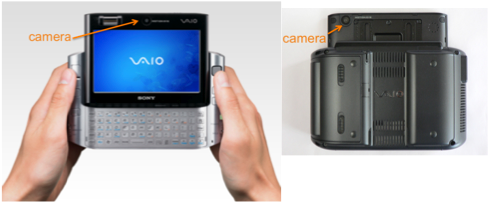
\includegraphics[width=14cm]{./Primitives/vaio.png}
	\rule{35em}{0.5pt}
	\caption[Sony VAIO VGN-UX90PS]{Sony VAIO VGN-UX90PS with a camera at the front and at the back}
	\label{fig:VAIO}
\end{figure}

This research aims to visualize the viewing fields of outdoor surveillance cameras on the screen of mobile devices. In this research, we propose:

\begin{itemize}
	\item Five methods to visualize viewing fields of surveillance cameras for outdoor MR.
	\item A new architecture of online camera calibration: server-side Parallel Tracking and Mapping (PTAM) \cite{Reference12} system. Our prototype system uses a mobile device which can be either a Sony VAIO VGN-UX90PS or an Apple iPhone and can provide realtime video. Because the mobile devices do not have sufficient computation facility to execute the heavy PTAM processing, we connect it wirelessly to a PTAM server which is an Apple MacBook Pro. This results in a system providing realtime MR video with no requirement for any GPS or gyrocompass devices.
\end{itemize}

Structure of this thesis:

\begin{itemize}
	\item Rest of chapter \ref{Chapter1} introduces the requirement on visualizing viewing fields of surveillance cameras, and some related technologies and researches.
	\item Chapter \ref{Chapter2} poses basic elements of visualization methods, then studies five visualization methods to show viewing fields of surveillance cameras.
	\item Chapter \ref{Chapter3} proposes online camera registration method based on server-side PTAM which implements and is integrated to the visualization methods in chapter \ref{Chapter2}.
	\item Chapter \ref{Chapter4} conducts an experiment to evaluate the five methods using the prototype, then discusses the result.
	\item Chapter \ref{Chapter5} summarizes this research and proposes future directions.
\end{itemize}

%------------------------------------------------------------------------------

\section{Use Case}
\label{UseCase}

When a user wants to see the visualized viewing fields of surrounding surveillance cameras on his own mobile device screen, the typical usage scenario is (see figure \ref{fig:UseCase} and \ref{fig:PrototypeArchitecture}):

\begin{enumerate}
	\item The user points the mobile camera in a certain direction.
	\item Through wireless network, the mobile device continuously sends video frames captured by the camera of the scene to a PTAM server.
	\item The PTAM server estimates the position and orientation of the mobile camera by analyzing the received video frames, and send them to the mobile device.
	\item Based on the position and orientation, the mobile device will correctly render visual aids that are instances of viewing fields of the surveillance cameras, and shows the MR video images on its screen.
	\item When the user changes the position or orientation of the mobile camera, the MR video displayed on the screen will simultaneously change accordingly to the camera movement.
\end{enumerate}

\begin{figure}[htbp]
	\centering
	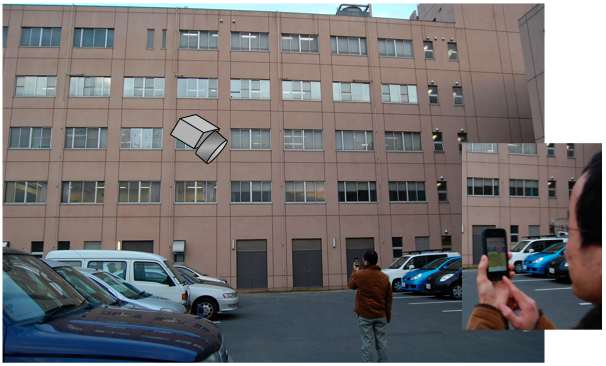
\includegraphics[width=14cm]{./Primitives/usecase.png}
	\rule{35em}{0.5pt}
	\caption[Usage scenario]{A usage scenario}
	\label{fig:UseCase}
\end{figure}

\begin{figure}[htbp]
	\centering
	\includegraphics[width=14cm]{./Figures/prototype_architecture.png}
	\rule{35em}{0.5pt}
	\caption[Prototype architecture]{Prototype architecture. The mobile device can be either a VAIO (appendix \ref{AppendixVAIO}) or an iPhone (appendix \ref{AppendixiPhone}).}
	\label{fig:PrototypeArchitecture}
\end{figure}

The above use case gives an example of the application of visualizing viewing fields of surveillance cameras and a rough idea of how the prototype works. There may be other applications. For example, we can build a system which visualizes ``safe paths'' or ``safe areas'' for children (figure \ref{fig:HomeSchool}). Children can use their cell phones to see if their current location is being well observed when they walk to school or back home.

\begin{figure}[htbp]
	\centering
	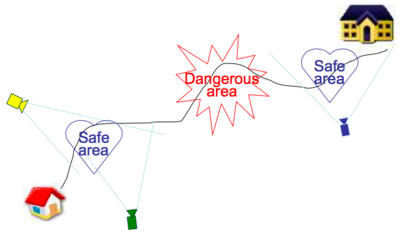
\includegraphics{./Primitives/home_school.png}
	\rule{35em}{0.5pt}
	\caption[Safe path to school]{Safe path to school}
	\label{fig:HomeSchool}
\end{figure}

%------------------------------------------------------------------------------

\section{Related Works}

For outdoor MR, bulky devices that reduce the mobility of users are not preferable. For example: heavy computers, devices wired to a fixed location, devices with big auxiliaries, big HMDs, HMDs that prevent users from seeing the outdoor environment while walking etc. Devices for outdoor MR should be small, lightweight, and can connect wirelessly to other devices if they need to.

MR systems usually need to know the position and orientation of the devices in order to merge images of the virtual world and the images of the real world at high accuracy. For indoor environment, marker-based solutions are known to work very well \cite{Reference20}. However, outdoor environment is usually large and it is impossible to put markers everywhere. There have been many researches that use UMPCs equipped with GPS and/or gyrocompass devices to realize markerless camera registration \cite{Reference2} \cite{Reference4} \cite{Reference13}. Hardware devices have been becoming smaller and more powerful according to Moore's law. Today's high-end cell phones, like Apple iPhone and Google T-Mobile G1, usually have built-in GPS and accelerometer devices. Because of their small size, high specifications, and competitive prices, such devices have found their use in outdoor MR applications and researches, like Sekai camera \cite{Reference18} and Enkin \cite{Reference19}.

However, normal GPS devices have error of about 5--10 m, and gyrocompass devices suffer from drift error. There have been many researches that are based on the images taken by the camera on the mobile device to deal with this problem. We can follow the approach that uses (1) gravity accelerometer to help eliminating the drift error, (2) model-based tracking on edges and (3) texture tracker to help produce accurate localization result \cite{Reference13}. There is also an approach that completely does not require GPS or gyrocompass devices, but uses the images taken by the camera and a landmark database of natural feature points built before-hand \cite{Reference21}.

When MR programs need more memory or CPU power than what the mobile devices can provide, we have a backup solution in which the mobile devices connect wirelessly to remote non-mobile computers to ask for help. It is possible to send realtime video images wirelessly to remote computers for further processing because 54 Mbps wireless network has become popular today. This may be a good approach because Moore's law has slowed down in recent years, thus we cannot expect the computation power of mobile devices to go much higher anytime soon while at the same time keeping their small size and mobility.
